% OLD
%\documentclass[11pt,compress,t,notes=noshow, aspectratio=169, xcolor=table]{beamer}
% new
\documentclass[10pt,compress,t,notes=noshow, xcolor=table]{beamer}

% OLD
%\usepackage{../../style/lmu-lecture}
% new
\input{../../style/preamble}
\input{../../latex-math/basic-ml}
\input{../../latex-math/basic-math}
% Defines macros and environments

\title{Interpretable Machine Learning}
% \author{LMU}
%\institute{\href{https://compstat-lmu.github.io/lectureml/}{compstat-lmu.github.io/lecture\ml}}

\begin{document}

% OLD
%\newcommand{\titlefigure}{figure/2023_paper_skizze_Planted_Tree.jpg}
%\newcommand{\learninggoals}{
%\item Motivation for RPFs
%\item Understand node types and restricting interactions in decision trees
%\item Understand planted trees: non-binary decision trees and inner leaves
%}
%
%\lecturechapter{Random Planted Forests}
%\lecture{Interpretable Machine Learning}
% new
\titlemeta{
Interpretable Models 2
}{
Random Planted Forests
}{
figure/2023_paper_skizze_Planted_Tree.jpg
}{
\item Motivation for RPFs
\item Understand node types and restricting interactions in decision trees
\item Understand planted trees: non-binary decision trees and inner leaves
}


%------------------------------------------------------------------
%------------------------------------------------------------------

\begin{framev}[align=top]{Random Planted Forests (RPF) % OLD
%\citebutton{Hiabu et al. 2023}{https://arxiv.org/abs/2012.14563}
% new
\furtherreading{HIABUETAL2023}}
\textbf{Goal:} Create a powerful tree ensemble, but still interpretable\\
\spacer[0.25]
\textbf{Idea:}
\begin{itemizeM}
\item GAMs easily interpretable, because no interaction $\leadsto$ plot 1D functions\\
\spacer[0.25]
\splitVCC[0.725]{
\spacer[0]
$$
\hat{f}(x) = \theta_0 + f_1(x_1) + f_2(x_2) + \ldots + f_p(x_p)
$$
\spacer[0]
}{
\spacer[0]
\imageC[0.8]{figure/gam_effects.pdf}
\spacer[0]
}
\item Same for functions containing interactions between max. 2 features\\
$\leadsto$ function of 2 features, plot 2D functions (i.e. 3D plot)
$$
\hat{f}(x) = \theta_0 + f_1(x_1) + f_2(x_2) + \ldots + f_p(x_p) + f_{1,2}(x_1, x_2) + \ldots + f_{1,p}(x_1, x_p) + \ldots + f_{p-1,p}(x_{p-1}, x_p)
$$
$\leadsto$ Visualize single functions $f_1$, $f_2$, $f_{1,2}(x_1, x_2)$, $f_{1,3}(x_1, x_3)$, $\ldots$
% TODO Also figures ?
\end{itemizeM}
$\Rightarrow$ Interpretability possible via restricting degree of interactions\\
\spacer[0.25]
\textbf{Problem:} How to know degree of interactions?\\
\spacer[0.25]
\textbf{Solution:} Easy to determine for trees / tree ensembles!
\end{framev}


\begin{framev}[align=top]{RPF: Determine interaction type in trees}
Define the \textit{interaction type $t$} of a node as the subset of features involved in constructing this node.\\
\spacer[0.25]
\textbf{Example:}
\begin{center}
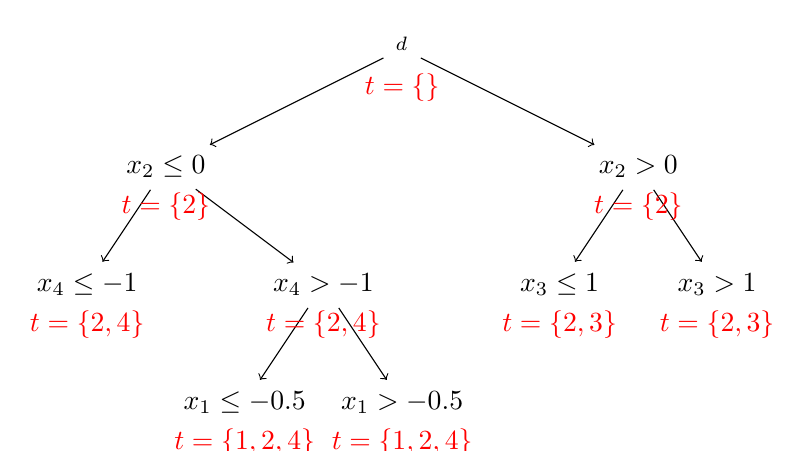
\begin{tikzpicture}[
node/.style = {scale=1},
scale = 1
]
        % \node[node] at (0,0)(root){\(x_2 \leq 0\)};
        %
        % \node[node] at (3,-1)(right_child){\(x_3 \leq 1\)};
        % \node[node] at (4,-2)(rightright_grandchild){$0.6$};
        % \node[node] at (2,-2)(rightleft_grandchild){\(-0.3\)};
        %
        % \node[node] at (-3,-1)(left_child){\(x_4 \leq -1\)};
        % \node[node] at (-4,-2)(leftleft_grandchild){$0.2$};
        % \node[node] at (-2,-2)(leftright_grandchild){\(x_1 \leq -0.5\)};
        %
        % \node[node] at (-2.5,-3)(low_child_1){$-0.1$};
        % \node[node] at (-1.5,-3)(low_child_2){$0.7$};
\node[node] at (0,2)(root){$\R^d$};
\node[node] at (3,.5)(right_child){$x_2 > 0$};
\node[node] at (4,-1)(rightright_grandchild){$x_3 > 1$};
\node[node] at (2,-1)(rightleft_grandchild){$x_3 \leq 1$};
\node[node] at (-3,.5)(left_child){$x_2 \leq 0$};
\node[node] at (-4,-1)(leftleft_grandchild){$x_4 \leq -1$};
\node[node] at (-1,-1)(leftright_grandchild){$x_4 > -1$};
\node[node] at (-2,-2.5)(low_child_1){$x_1 \leq -0.5$};
\node[node] at (0,-2.5)(low_child_2){$x_1 > -0.5$};
\draw[->, shorten >= 1pt, shorten <= 1pt] (root) -- (left_child);
\draw[->, shorten >= 1pt, shorten <= 1pt] (root) -- (right_child);
\draw[->, shorten >= 1pt, shorten <= 1pt] (left_child) -- (leftleft_grandchild);
\draw[->, shorten >= 1pt, shorten <= 1pt] (left_child) -- (leftright_grandchild);
\draw[->, shorten >= 1pt, shorten <= 1pt] (right_child) -- (rightright_grandchild);
\draw[->, shorten >= 1pt, shorten <= 1pt] (right_child) -- (rightleft_grandchild);
\draw[->, shorten >= 1pt, shorten <= 1pt] (leftright_grandchild) -- (low_child_1);
\draw[->, shorten >= 1pt, shorten <= 1pt] (leftright_grandchild) -- (low_child_2);
\only<2>{
\node[overlay, node, color=red] at (0,1.5)(root_type){$t=\{\}$};
\node[overlay, node, color=red] at (3,0)(right_child_type){$t=\{2\}$};
\node[overlay, node, color=red] at (4,-1.5)(rightright_grandchild_type){$t=\{2,3\}$};
\node[overlay, node, color=red] at (2,-1.5)(rightleft_grandchild_type){$t=\{2,3\}$};
\node[overlay, node, color=red] at (-3,0)(left_child_type){$t=\{2\}$};
\node[overlay, node, color=red] at (-4,-1.5)(leftleft_grandchild_type){$t=\{2,4\}$};
\node[overlay, node, color=red] at (-1,-1.5)(leftright_grandchild_type){$t=\{2,4\}$};
\node[overlay, node, color=red] at (-2,-3)(low_child_1_type){$t=\{1,2,4\}$};
\node[overlay, node, color=red] at (0,-3)(low_child_2_type){$t=\{1,2,4\}$};
        % \draw (-2,-3.3) ellipse (1.1cm and 0.6cm);
        % \draw (0,0) ellipse (2cm and 1cm);
}
\end{tikzpicture}
\end{center}
% use of \spacer[1] since it doesn't look good with \spacer[0.25]
\spacer[1]
\only<2>{
$\Rightarrow$ Degree of interaction in each node is \(|t|\).
}
\end{framev}


\begin{framev}[align=top]{RPF: bounded interaction order + Planted trees}
\textbf{Goal}: restrict this interaction degree\\
$\leadsto$ In RPFs:
\begin{itemizeM}
\item Always keep track of the interaction type in each node
\item For each new split, make sure the max. degree of interactions is not exceeded\\ $\Rightarrow$ When max. number of feat reached, no new feat are allowed
\end{itemizeM}
\spacer[0.25]
\textbf{Problem:} For small interaction order, single trees quickly become limited
\begin{itemizeM}
\item E.g. interaction order 1: every tree uses only one feature
\item[$\Rightarrow$] Many trees are needed for a more complex model
\end{itemizeM}

\spacer[0.25]
\textbf{Idea:} Allow inner nodes to split again\\
\spacer[0.25]
Define \textit{Planted Trees}: decision trees where each inner node can be a \textit{leaf}:
\begin{itemizeM}
\item Add prediction to final output
\item Can be split again $\Rightarrow$ several splits possible
\end{itemizeM}
\end{framev}

% \begin{frame}{RPF: Example}

%     \begin{figure}[h]
%         \centering
%         % \vspace{-10pt} % Note that this is only to ensure a normal, not to big margin around the figure
%         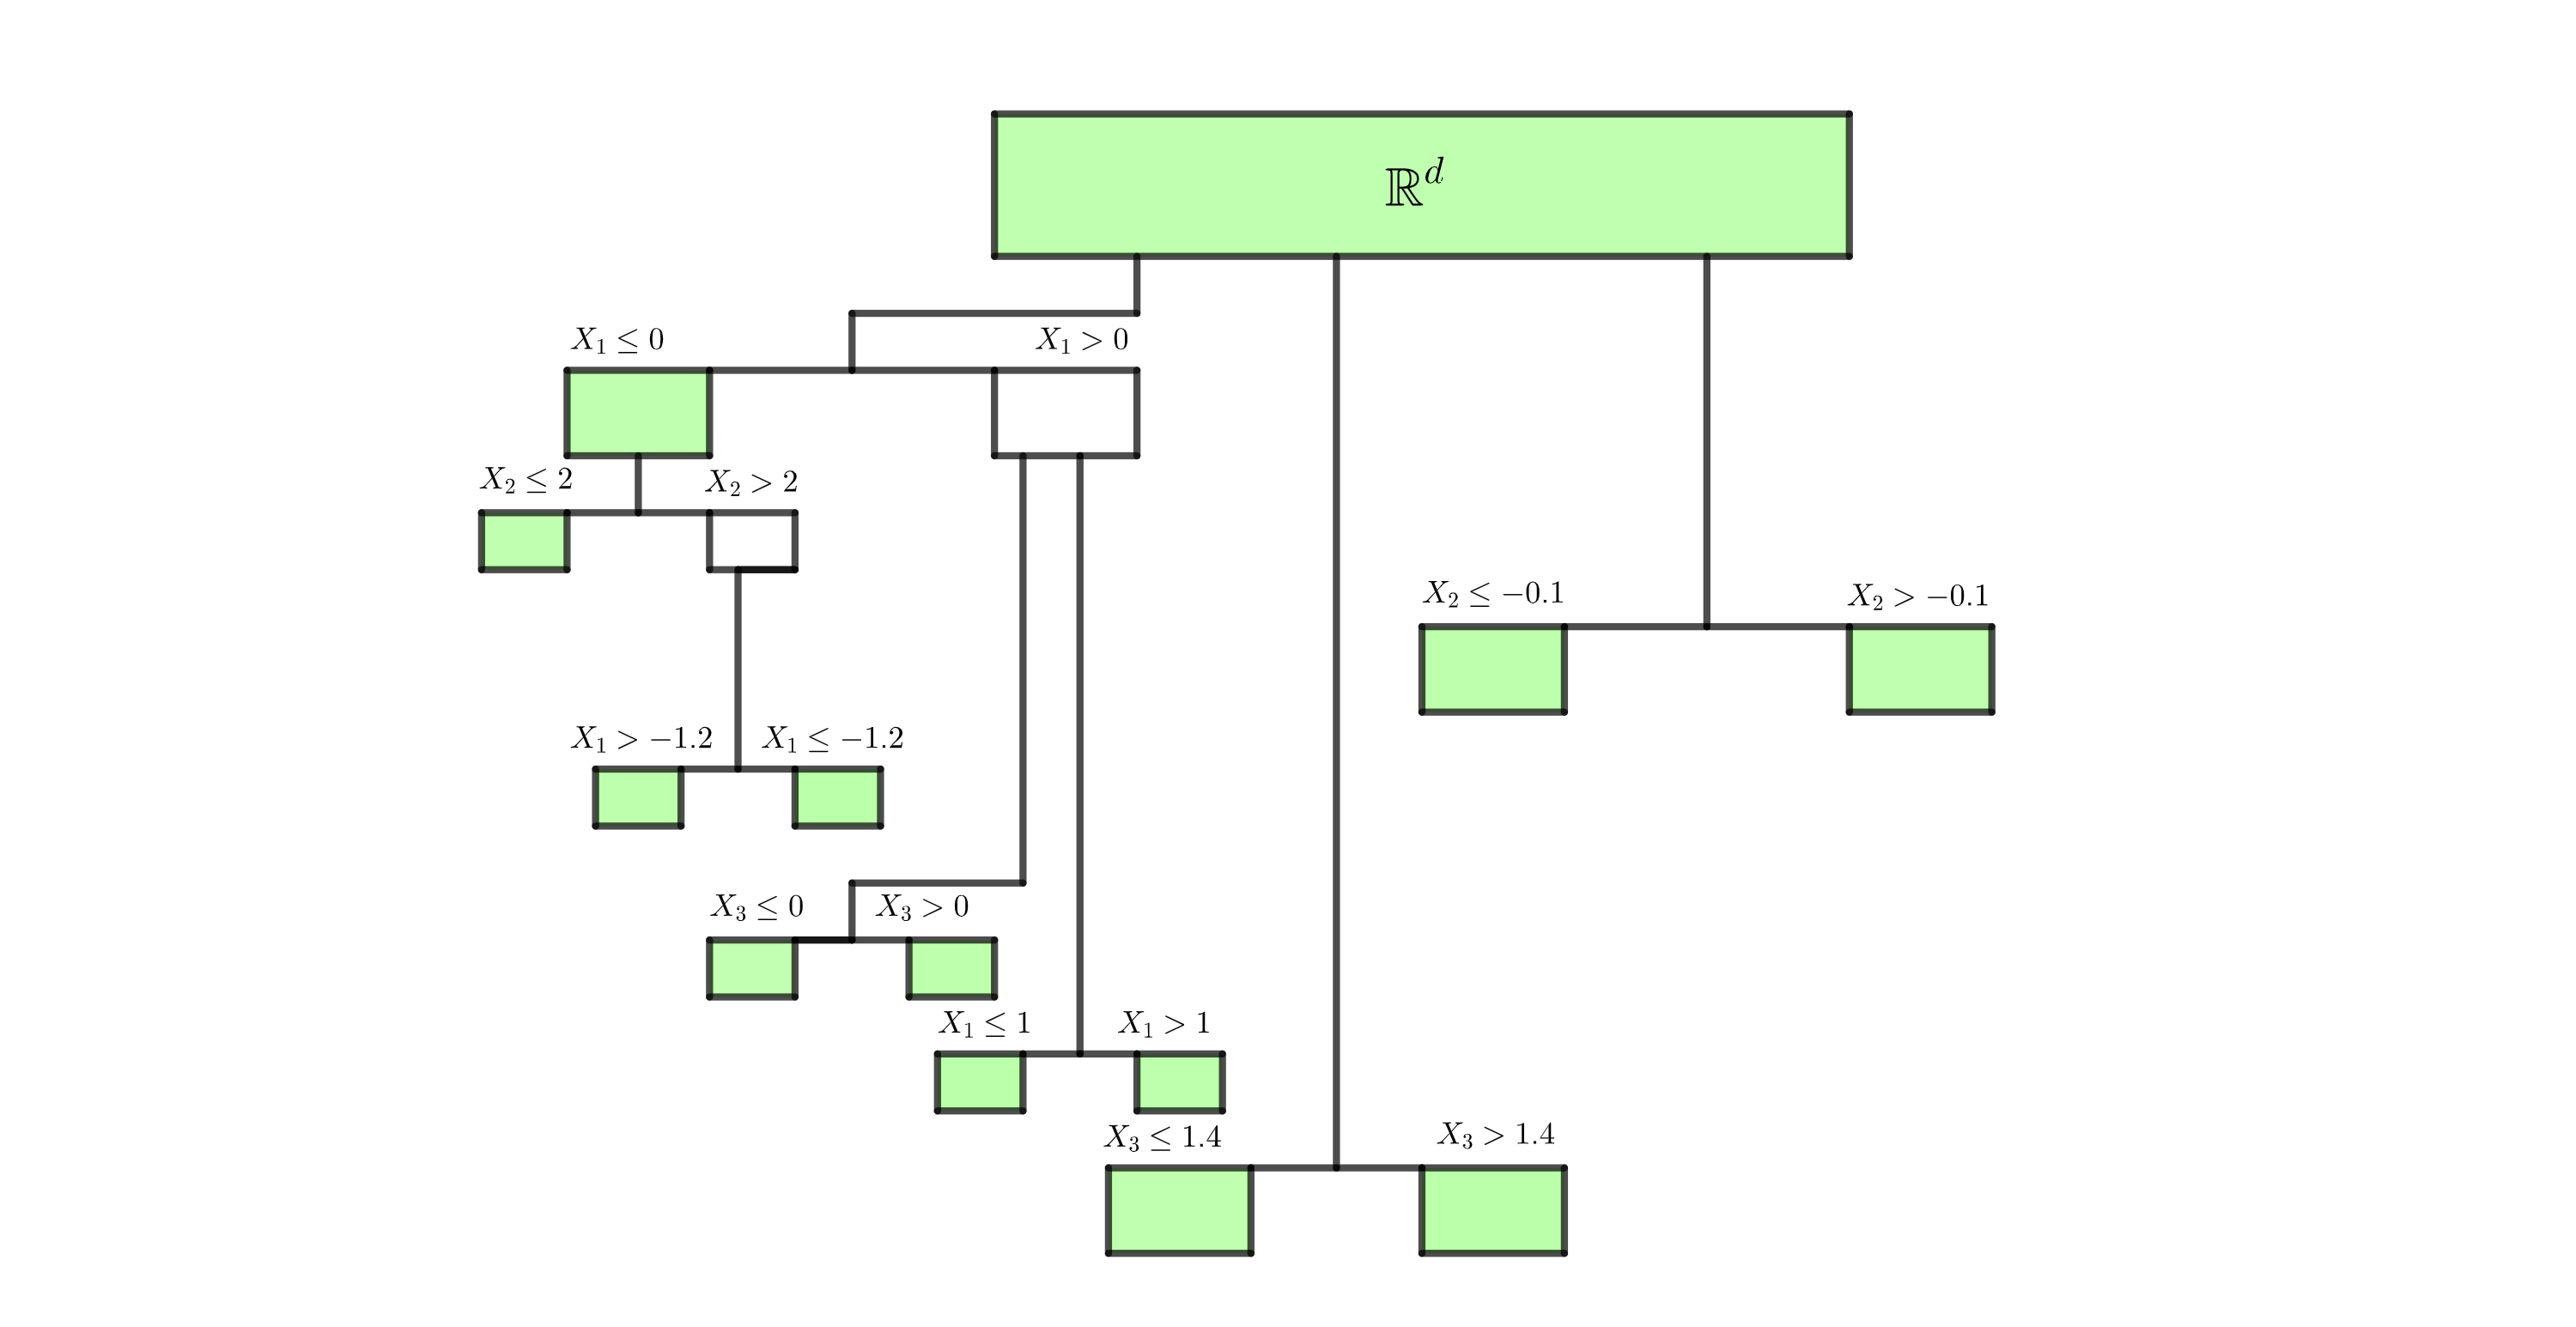
\includegraphics[width=1.1\linewidth]{figure/2023_paper_skizze_Planted_Tree.jpg}
%         % \vspace{-10pt}
%         \caption{Example of a single fully grown planted tree}
%         \label{fig:Planted_Tree_example_paper}
%     \end{figure}

% \end{frame}

\begin{framev}[align=top]{RPF: Example}
\begin{center}
\begin{figure}[h]
\begin{tikzpicture}[
node/.style = {scale=.5},
scale = 1
]
\node[anchor=south west,inner sep=0] (image) at (0,0) {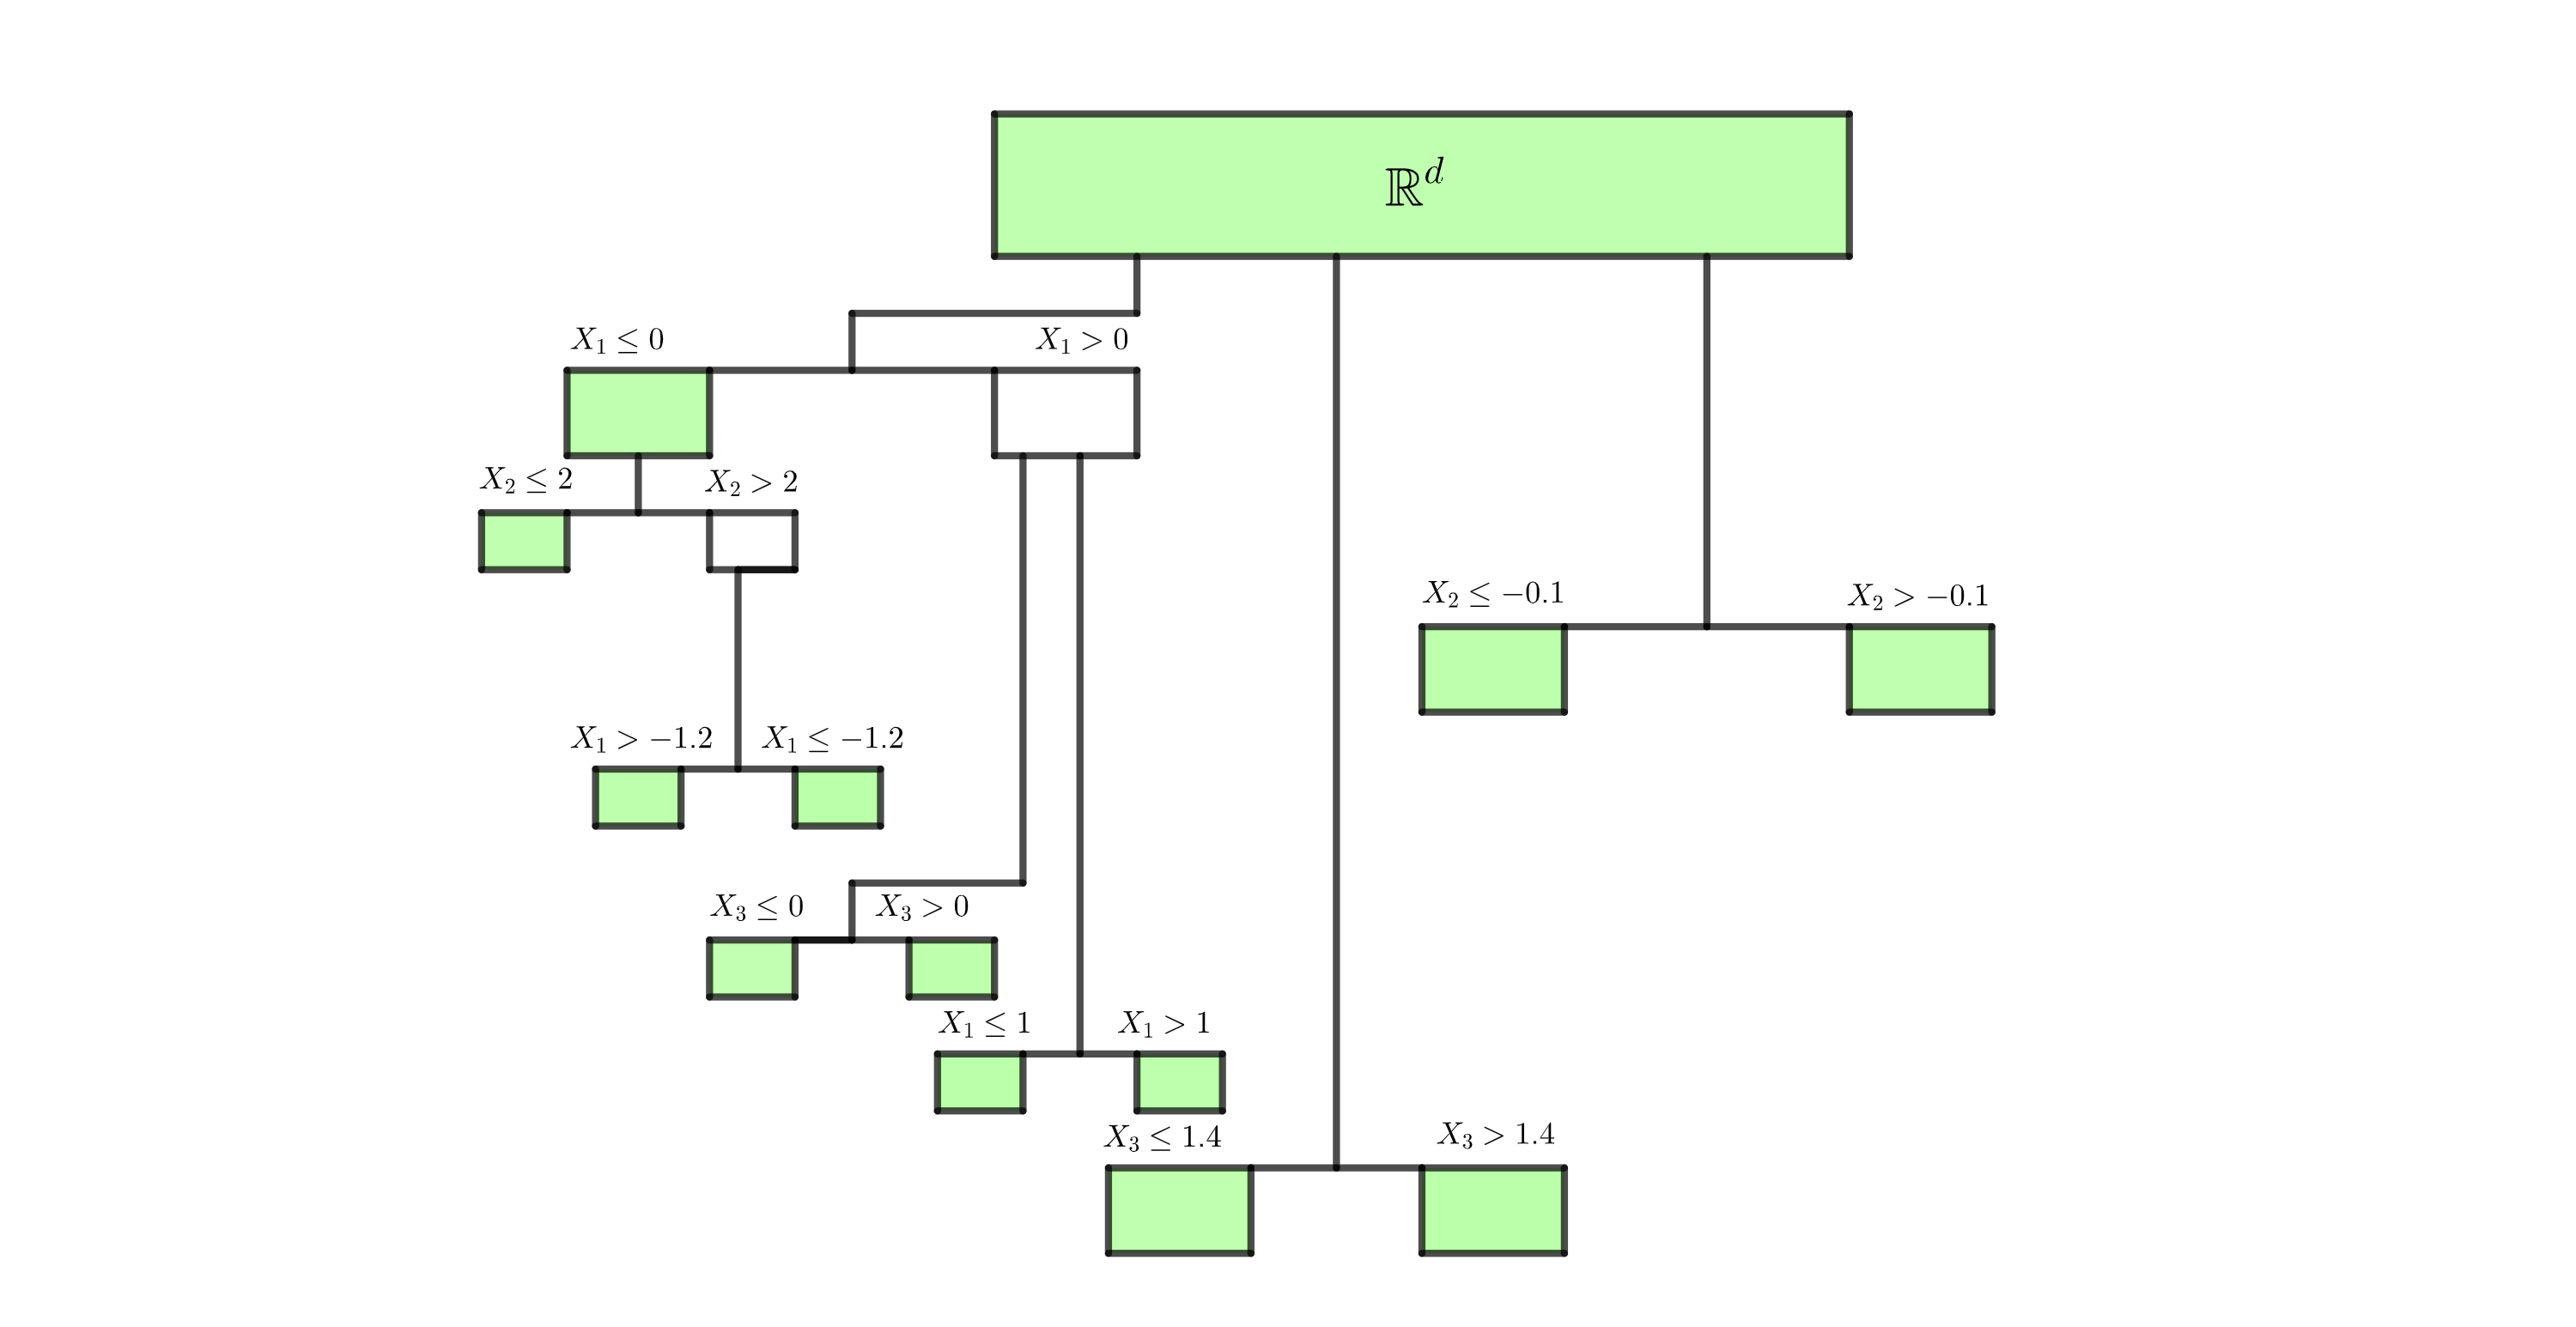
\includegraphics[width=1.1\linewidth]{figure/2023_paper_skizze_Planted_Tree.jpg}};
\only<2>{
\node[node, color=red] at (8,6)(root_type){$t=\{\}$};
\node[node, color=red] at (3.35,4.8)(leftleft_type){$\{1\}$};
\node[node, color=red] at (5.55,4.8)(leftright_type){$\{1\}$};
\node[node, color=red] at (3.95,4.1)(leftleft_right_type){$\{1,2\}$};
\node[node, color=red] at (2.75,4.1)(leftleft_left_type){$\{1,2\}$};
\node[node, color=red] at (3.35,2.8)(leftleft_right_left_type){$\{1,2\}$};
\node[node, color=red] at (4.35,2.8)(leftleft_right_right_type){$\{1,2\}$};
\node[node, color=red] at (3.95,1.9)(leftright_leftleft_type){$\{1,3\}$};
\node[node, color=red] at (4.95,1.9)(leftright_leftright_type){$\{1,3\}$};
        % \node[node, color=red] at (5,1)(left_right_type_dummy){$\{1\}$};
\node[node, color=red] at (5.15,1.25)(leftright_rightleft_type){$\{1\}$};
\node[node, color=red] at (6.15,1.25)(leftright_rightright_type){$\{1\}$};
\node[node, color=red] at (7.75,.65)(midright_type){$\{3\}$};
\node[node, color=red] at (6.15,.65)(midleft_type){$\{3\}$};
}
\end{tikzpicture}
\caption{Example of a single fully grown planted tree, green nodes: ``leaves''}
\label{fig:Planted_Tree_example_paper}
\end{figure}
\end{center}
\end{framev}


\begin{framei}[align=top]{RPF: Algo}
\item Max. interaction degree is a hyperparameter
\item Total number of trees is a hyperparameter
\item End growing tree after the maximum total number of splits instead of the maximum depth\\
(Minimum number of samples is also possible, but then higher nodes would split too often)
\item Randomization as in random forests:
\begin{itemizeS}
\item Only optimize over a randomly chosen subset of features
\item Only optimize over a subset of possible split values
\end{itemizeS}
\item Make an inner leaf an inner node (i.e.\ delete the ``leaf'' property) if it has children with the same type
\end{framei}


\begin{framev}[align=top]{RPF: Example results and interpretation}
\end{framev}


\begin{framev}[align=top]{RPF: Conclusion}
\end{framev}

\endlecture
\end{document}
